\hypertarget{S3Classes_8c}{
\section{S3Classes.c File Reference}
\label{S3Classes_8c}\index{S3Classes.c@{S3Classes.c}}
}
{\tt \#include \char`\"{}party.h\char`\"{}}\par


Include dependency graph for S3Classes.c:\begin{figure}[H]
\begin{center}
\leavevmode
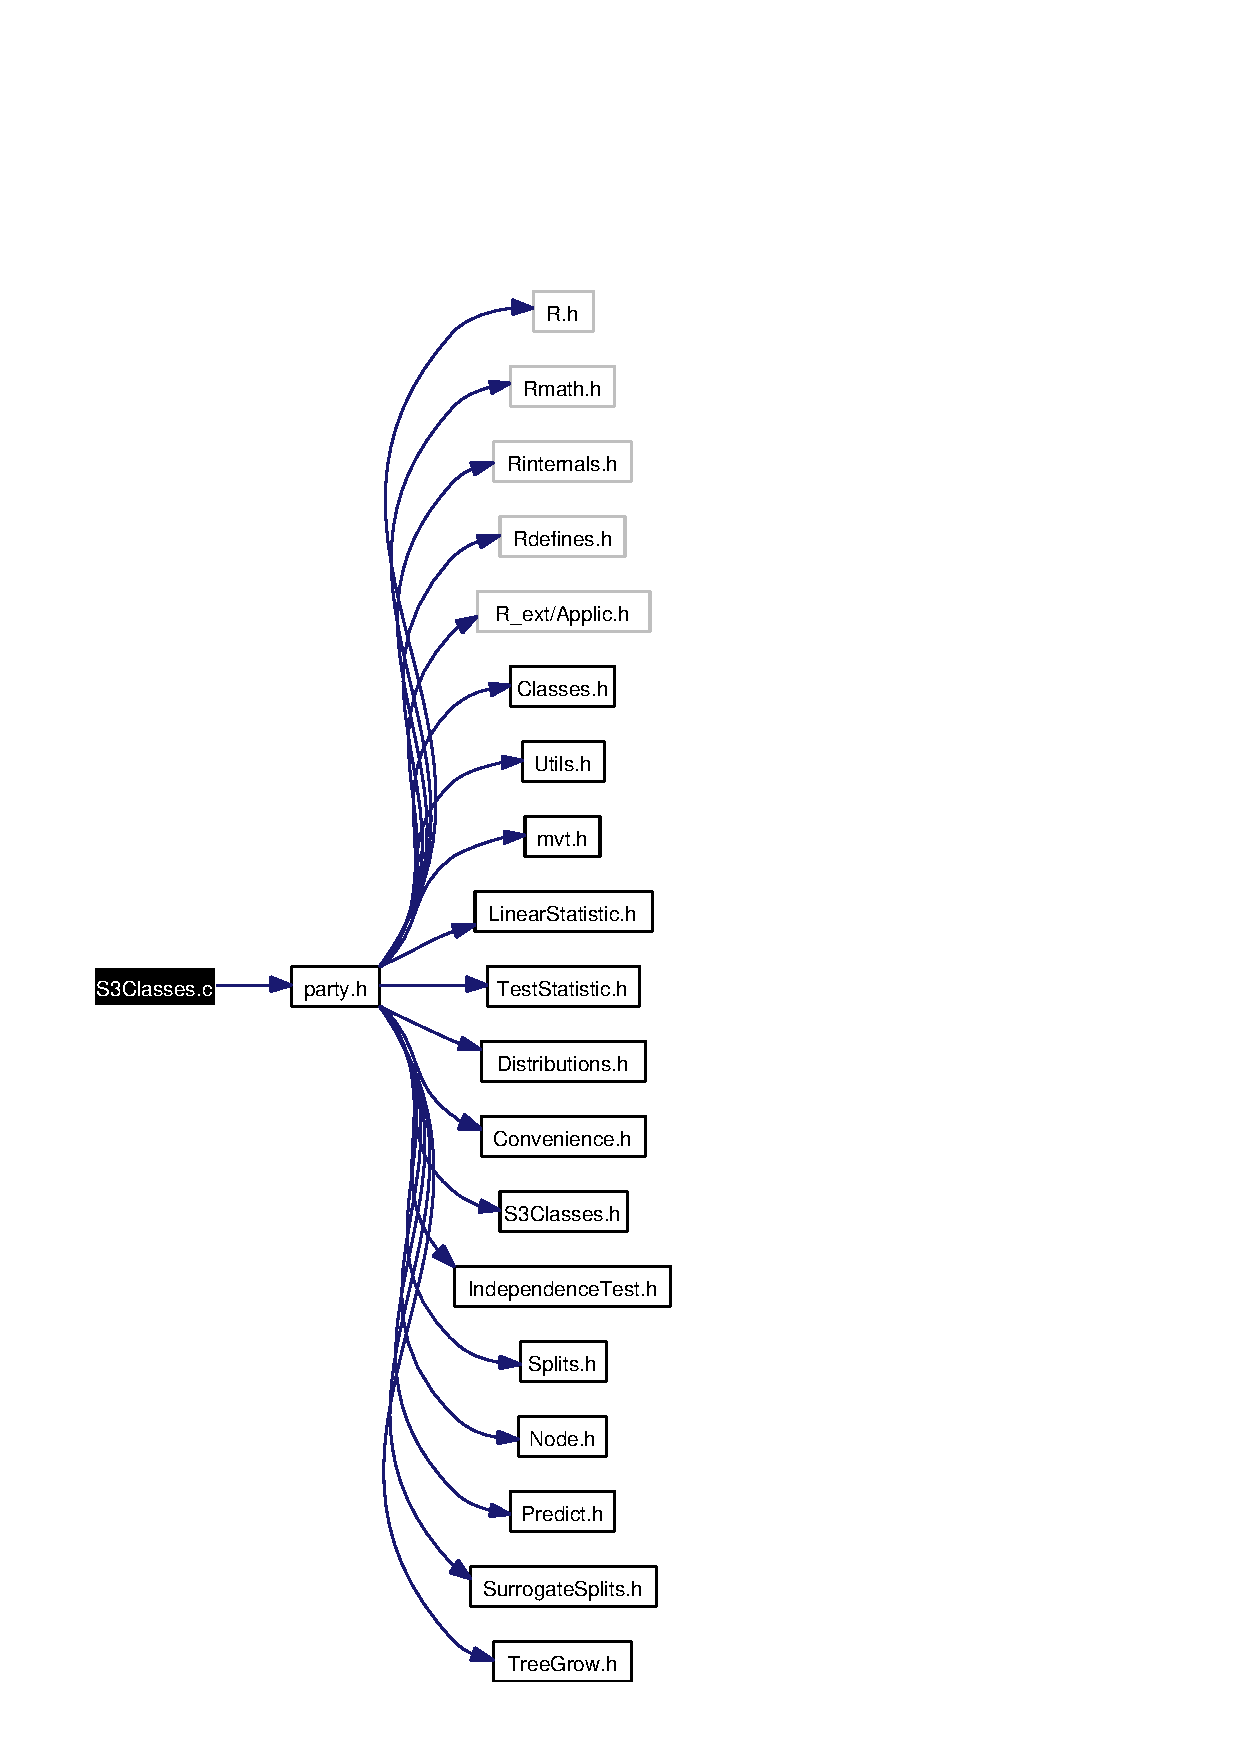
\includegraphics[width=168pt]{S3Classes_8c__incl}
\end{center}
\end{figure}
\subsection*{Functions}
\begin{CompactItemize}
\item 
void \hyperlink{S3Classes_8c_f837f0cf74c62c53c74138c4dbb9acc0}{C\_\-init\_\-node} (SEXP node, int nobs, int ninputs, int nsurr, int q)
\item 
void \hyperlink{S3Classes_8c_3130204036068f194e66d7f8b39da73c}{S3set\_\-node\-ID} (SEXP node, int node\-ID)
\item 
int \hyperlink{S3Classes_8c_136b05ff188fc291196cc9d37d52e862}{S3get\_\-node\-ID} (SEXP node)
\item 
SEXP \hyperlink{S3Classes_8c_c3785782483b5bf4afe9d606e280f3ca}{S3get\_\-nodeweights} (SEXP node)
\item 
double \hyperlink{S3Classes_8c_d5b760cf2b547dc128273948f78b7a3c}{S3get\_\-sumweights} (SEXP node)
\item 
SEXP \hyperlink{S3Classes_8c_174b61cf01697f1693e14e449611563c}{S3get\_\-teststat} (SEXP node)
\item 
SEXP \hyperlink{S3Classes_8c_7e1195f9e99aa93145f04e80c62ff687}{S3get\_\-criterion} (SEXP node)
\item 
SEXP \hyperlink{S3Classes_8c_e5d3e3ccef4e5fbfe1b6cf683b4d2999}{S3get\_\-maxcriterion} (SEXP node)
\item 
void \hyperlink{S3Classes_8c_81cae2a178f2bb5562a12c974d966add}{S3set\_\-nodeterminal} (SEXP node)
\item 
int \hyperlink{S3Classes_8c_b8834f319068d2a248a5d6328cd10dc5}{S3get\_\-nodeterminal} (SEXP node)
\item 
SEXP \hyperlink{S3Classes_8c_220373298b30f12b22f82cce3c996a37}{S3get\_\-primarysplit} (SEXP node)
\item 
SEXP \hyperlink{S3Classes_8c_f270d1d02bf86a4c5cdc8959045c3567}{S3get\_\-surrogatesplits} (SEXP node)
\item 
SEXP \hyperlink{S3Classes_8c_70a340b301b4e383107c92cbbeb4ae20}{S3get\_\-prediction} (SEXP node)
\item 
SEXP \hyperlink{S3Classes_8c_5917f57e141432fd1e4f58a16b9149aa}{S3get\_\-leftnode} (SEXP node)
\item 
SEXP \hyperlink{S3Classes_8c_14a38e81ed758a64367dc190f0e8229b}{S3get\_\-rightnode} (SEXP node)
\item 
void \hyperlink{S3Classes_8c_c727b2483cf36cd256889ac9f8203258}{C\_\-init\_\-orderedsplit} (SEXP split, int nobs)
\item 
void \hyperlink{S3Classes_8c_07230eaacca448a8235ea7760adbfa04}{C\_\-init\_\-nominalsplit} (SEXP split, int nlevels, int nobs)
\item 
void \hyperlink{S3Classes_8c_06ea5a46f63ebc5c27c005610dc6f8fc}{S3set\_\-variable\-ID} (SEXP split, int variable\-ID)
\item 
int \hyperlink{S3Classes_8c_583f9148949f93b5fe894feb6567ca0d}{S3get\_\-variable\-ID} (SEXP split)
\item 
int \hyperlink{S3Classes_8c_54ed9f6b46c69d550ceea1a525287ecf}{S3is\_\-ordered} (SEXP split)
\item 
void \hyperlink{S3Classes_8c_db2e0a52bc6a8eb0c74449942777d1a1}{S3set\_\-ordered} (SEXP split)
\item 
void \hyperlink{S3Classes_8c_abc3b50bbc29acb0b2c7ac0ed42fcb56}{S3set\_\-nominal} (SEXP split)
\item 
int \hyperlink{S3Classes_8c_67d50b82dea660a930cf7427be899efb}{S3get\_\-toleft} (SEXP split)
\item 
void \hyperlink{S3Classes_8c_c092009b36513086514bbe7aff516f12}{S3set\_\-toleft} (SEXP split, int left)
\item 
SEXP \hyperlink{S3Classes_8c_acf87d496fd3b07bafd171c92404212a}{S3get\_\-splitpoint} (SEXP split)
\item 
SEXP \hyperlink{S3Classes_8c_a22b5c06c2e2e7ad8bf873df35a8bb99}{S3get\_\-splitstatistics} (SEXP split)
\item 
SEXP \hyperlink{S3Classes_8c_ab4c2cafa901e0303b662c1b1542099a}{S3get\_\-table} (SEXP split)
\end{CompactItemize}


\subsection{Detailed Description}
S3 classes for dealing with nodes and splits

\begin{Desc}
\item[Author:]\begin{Desc}
\item[Author]hothorn \end{Desc}
\end{Desc}
\begin{Desc}
\item[Date:]\begin{Desc}
\item[Date]2007-07-23 09:44:00 +0200 (Mon, 23 Jul 2007) \end{Desc}
\end{Desc}


Definition in file \hyperlink{S3Classes_8c-source}{S3Classes.c}.

\subsection{Function Documentation}
\hypertarget{S3Classes_8c_f837f0cf74c62c53c74138c4dbb9acc0}{
\index{S3Classes.c@{S3Classes.c}!C_init_node@{C\_\-init\_\-node}}
\index{C_init_node@{C\_\-init\_\-node}!S3Classes.c@{S3Classes.c}}
\subsubsection[C\_\-init\_\-node]{\setlength{\rightskip}{0pt plus 5cm}void C\_\-init\_\-node (SEXP {\em node}, int {\em nobs}, int {\em ninputs}, int {\em nsurr}, int {\em q})}}
\label{S3Classes_8c_f837f0cf74c62c53c74138c4dbb9acc0}




Definition at line 11 of file S3Classes.c.

References CRITERION\_\-LENGTH, NODE\_\-LENGTH, S3\_\-CRITERION, S3\_\-i\-CRITERION, S3\_\-MAXCRITERION, S3\_\-NODEID, S3\_\-PREDICTION, S3\_\-PSPLIT, S3\_\-SSPLIT, S3\_\-STATISTICS, S3\_\-SUMWEIGHTS, S3\_\-TERMINAL, S3\_\-WEIGHTS, and SPLIT\_\-LENGTH.

Referenced by C\_\-splitnode(), R\_\-Node(), and R\_\-Tree\-Grow().\hypertarget{S3Classes_8c_07230eaacca448a8235ea7760adbfa04}{
\index{S3Classes.c@{S3Classes.c}!C_init_nominalsplit@{C\_\-init\_\-nominalsplit}}
\index{C_init_nominalsplit@{C\_\-init\_\-nominalsplit}!S3Classes.c@{S3Classes.c}}
\subsubsection[C\_\-init\_\-nominalsplit]{\setlength{\rightskip}{0pt plus 5cm}void C\_\-init\_\-nominalsplit (SEXP {\em split}, int {\em nlevels}, int {\em nobs})}}
\label{S3Classes_8c_07230eaacca448a8235ea7760adbfa04}




Definition at line 128 of file S3Classes.c.

References S3\_\-ORDERED, S3\_\-SPLITPOINT, S3\_\-SPLITSTATISTICS, S3\_\-TABLE, S3\_\-TOLEFT, S3\_\-VARIABLEID, and SPLIT\_\-LENGTH.

Referenced by C\_\-Node().\hypertarget{S3Classes_8c_c727b2483cf36cd256889ac9f8203258}{
\index{S3Classes.c@{S3Classes.c}!C_init_orderedsplit@{C\_\-init\_\-orderedsplit}}
\index{C_init_orderedsplit@{C\_\-init\_\-orderedsplit}!S3Classes.c@{S3Classes.c}}
\subsubsection[C\_\-init\_\-orderedsplit]{\setlength{\rightskip}{0pt plus 5cm}void C\_\-init\_\-orderedsplit (SEXP {\em split}, int {\em nobs})}}
\label{S3Classes_8c_c727b2483cf36cd256889ac9f8203258}




Definition at line 104 of file S3Classes.c.

References S3\_\-ORDERED, S3\_\-SPLITPOINT, S3\_\-SPLITSTATISTICS, S3\_\-TABLE, S3\_\-TOLEFT, S3\_\-VARIABLEID, and SPLIT\_\-LENGTH.

Referenced by C\_\-Node().\hypertarget{S3Classes_8c_7e1195f9e99aa93145f04e80c62ff687}{
\index{S3Classes.c@{S3Classes.c}!S3get_criterion@{S3get\_\-criterion}}
\index{S3get_criterion@{S3get\_\-criterion}!S3Classes.c@{S3Classes.c}}
\subsubsection[S3get\_\-criterion]{\setlength{\rightskip}{0pt plus 5cm}SEXP S3get\_\-criterion (SEXP {\em node})}}
\label{S3Classes_8c_7e1195f9e99aa93145f04e80c62ff687}




Definition at line 68 of file S3Classes.c.

References S3\_\-CRITERION, and S3\_\-i\-CRITERION.

Referenced by C\_\-Node().\hypertarget{S3Classes_8c_5917f57e141432fd1e4f58a16b9149aa}{
\index{S3Classes.c@{S3Classes.c}!S3get_leftnode@{S3get\_\-leftnode}}
\index{S3get_leftnode@{S3get\_\-leftnode}!S3Classes.c@{S3Classes.c}}
\subsubsection[S3get\_\-leftnode]{\setlength{\rightskip}{0pt plus 5cm}SEXP S3get\_\-leftnode (SEXP {\em node})}}
\label{S3Classes_8c_5917f57e141432fd1e4f58a16b9149aa}




Definition at line 96 of file S3Classes.c.

References S3\_\-LEFT.

Referenced by C\_\-get\_\-node(), C\_\-get\_\-nodebynum(), C\_\-remove\_\-weights(), C\_\-splitsurrogate(), and C\_\-Tree\-Grow().\hypertarget{S3Classes_8c_e5d3e3ccef4e5fbfe1b6cf683b4d2999}{
\index{S3Classes.c@{S3Classes.c}!S3get_maxcriterion@{S3get\_\-maxcriterion}}
\index{S3get_maxcriterion@{S3get\_\-maxcriterion}!S3Classes.c@{S3Classes.c}}
\subsubsection[S3get\_\-maxcriterion]{\setlength{\rightskip}{0pt plus 5cm}SEXP S3get\_\-maxcriterion (SEXP {\em node})}}
\label{S3Classes_8c_e5d3e3ccef4e5fbfe1b6cf683b4d2999}




Definition at line 72 of file S3Classes.c.

References S3\_\-CRITERION, and S3\_\-MAXCRITERION.

Referenced by C\_\-get\_\-node(), and C\_\-Node().\hypertarget{S3Classes_8c_136b05ff188fc291196cc9d37d52e862}{
\index{S3Classes.c@{S3Classes.c}!S3get_nodeID@{S3get\_\-nodeID}}
\index{S3get_nodeID@{S3get\_\-nodeID}!S3Classes.c@{S3Classes.c}}
\subsubsection[S3get\_\-nodeID]{\setlength{\rightskip}{0pt plus 5cm}int S3get\_\-node\-ID (SEXP {\em node})}}
\label{S3Classes_8c_136b05ff188fc291196cc9d37d52e862}




Definition at line 47 of file S3Classes.c.

References S3\_\-NODEID.

Referenced by C\_\-get\_\-nodebynum(), and C\_\-get\_\-node\-ID().\hypertarget{S3Classes_8c_b8834f319068d2a248a5d6328cd10dc5}{
\index{S3Classes.c@{S3Classes.c}!S3get_nodeterminal@{S3get\_\-nodeterminal}}
\index{S3get_nodeterminal@{S3get\_\-nodeterminal}!S3Classes.c@{S3Classes.c}}
\subsubsection[S3get\_\-nodeterminal]{\setlength{\rightskip}{0pt plus 5cm}int S3get\_\-nodeterminal (SEXP {\em node})}}
\label{S3Classes_8c_b8834f319068d2a248a5d6328cd10dc5}




Definition at line 80 of file S3Classes.c.

References S3\_\-TERMINAL.

Referenced by C\_\-get\_\-node(), C\_\-get\_\-nodebynum(), C\_\-remove\_\-weights(), and C\_\-Tree\-Grow().\hypertarget{S3Classes_8c_c3785782483b5bf4afe9d606e280f3ca}{
\index{S3Classes.c@{S3Classes.c}!S3get_nodeweights@{S3get\_\-nodeweights}}
\index{S3get_nodeweights@{S3get\_\-nodeweights}!S3Classes.c@{S3Classes.c}}
\subsubsection[S3get\_\-nodeweights]{\setlength{\rightskip}{0pt plus 5cm}SEXP S3get\_\-nodeweights (SEXP {\em node})}}
\label{S3Classes_8c_c3785782483b5bf4afe9d606e280f3ca}




Definition at line 51 of file S3Classes.c.

References S3\_\-WEIGHTS.

Referenced by C\_\-get\_\-nodeweights(), C\_\-splitnode(), C\_\-splitsurrogate(), C\_\-surrogates(), C\_\-Tree\-Grow(), and R\_\-Tree\-Grow().\hypertarget{S3Classes_8c_70a340b301b4e383107c92cbbeb4ae20}{
\index{S3Classes.c@{S3Classes.c}!S3get_prediction@{S3get\_\-prediction}}
\index{S3get_prediction@{S3get\_\-prediction}!S3Classes.c@{S3Classes.c}}
\subsubsection[S3get\_\-prediction]{\setlength{\rightskip}{0pt plus 5cm}SEXP S3get\_\-prediction (SEXP {\em node})}}
\label{S3Classes_8c_70a340b301b4e383107c92cbbeb4ae20}




Definition at line 92 of file S3Classes.c.

References S3\_\-PREDICTION.

Referenced by C\_\-get\_\-prediction(), C\_\-getpredictions(), C\_\-Node(), and R\_\-predict\-RF\_\-weights().\hypertarget{S3Classes_8c_220373298b30f12b22f82cce3c996a37}{
\index{S3Classes.c@{S3Classes.c}!S3get_primarysplit@{S3get\_\-primarysplit}}
\index{S3get_primarysplit@{S3get\_\-primarysplit}!S3Classes.c@{S3Classes.c}}
\subsubsection[S3get\_\-primarysplit]{\setlength{\rightskip}{0pt plus 5cm}SEXP S3get\_\-primarysplit (SEXP {\em node})}}
\label{S3Classes_8c_220373298b30f12b22f82cce3c996a37}




Definition at line 84 of file S3Classes.c.

References S3\_\-PSPLIT.

Referenced by C\_\-get\_\-node(), C\_\-Node(), C\_\-splitnode(), C\_\-splitsurrogate(), and C\_\-surrogates().\hypertarget{S3Classes_8c_14a38e81ed758a64367dc190f0e8229b}{
\index{S3Classes.c@{S3Classes.c}!S3get_rightnode@{S3get\_\-rightnode}}
\index{S3get_rightnode@{S3get\_\-rightnode}!S3Classes.c@{S3Classes.c}}
\subsubsection[S3get\_\-rightnode]{\setlength{\rightskip}{0pt plus 5cm}SEXP S3get\_\-rightnode (SEXP {\em node})}}
\label{S3Classes_8c_14a38e81ed758a64367dc190f0e8229b}




Definition at line 100 of file S3Classes.c.

References S3\_\-RIGHT.

Referenced by C\_\-get\_\-node(), C\_\-get\_\-nodebynum(), C\_\-remove\_\-weights(), C\_\-splitsurrogate(), and C\_\-Tree\-Grow().\hypertarget{S3Classes_8c_acf87d496fd3b07bafd171c92404212a}{
\index{S3Classes.c@{S3Classes.c}!S3get_splitpoint@{S3get\_\-splitpoint}}
\index{S3get_splitpoint@{S3get\_\-splitpoint}!S3Classes.c@{S3Classes.c}}
\subsubsection[S3get\_\-splitpoint]{\setlength{\rightskip}{0pt plus 5cm}SEXP S3get\_\-splitpoint (SEXP {\em split})}}
\label{S3Classes_8c_acf87d496fd3b07bafd171c92404212a}




Definition at line 179 of file S3Classes.c.

References S3\_\-SPLITPOINT.

Referenced by C\_\-get\_\-node(), C\_\-Node(), C\_\-splitnode(), and C\_\-splitsurrogate().\hypertarget{S3Classes_8c_a22b5c06c2e2e7ad8bf873df35a8bb99}{
\index{S3Classes.c@{S3Classes.c}!S3get_splitstatistics@{S3get\_\-splitstatistics}}
\index{S3get_splitstatistics@{S3get\_\-splitstatistics}!S3Classes.c@{S3Classes.c}}
\subsubsection[S3get\_\-splitstatistics]{\setlength{\rightskip}{0pt plus 5cm}SEXP S3get\_\-splitstatistics (SEXP {\em split})}}
\label{S3Classes_8c_a22b5c06c2e2e7ad8bf873df35a8bb99}




Definition at line 183 of file S3Classes.c.

References S3\_\-SPLITSTATISTICS.

Referenced by C\_\-Node().\hypertarget{S3Classes_8c_d5b760cf2b547dc128273948f78b7a3c}{
\index{S3Classes.c@{S3Classes.c}!S3get_sumweights@{S3get\_\-sumweights}}
\index{S3get_sumweights@{S3get\_\-sumweights}!S3Classes.c@{S3Classes.c}}
\subsubsection[S3get\_\-sumweights]{\setlength{\rightskip}{0pt plus 5cm}double S3get\_\-sumweights (SEXP {\em node})}}
\label{S3Classes_8c_d5b760cf2b547dc128273948f78b7a3c}




Definition at line 60 of file S3Classes.c.

References S3\_\-SUMWEIGHTS.

Referenced by C\_\-get\_\-node().\hypertarget{S3Classes_8c_f270d1d02bf86a4c5cdc8959045c3567}{
\index{S3Classes.c@{S3Classes.c}!S3get_surrogatesplits@{S3get\_\-surrogatesplits}}
\index{S3get_surrogatesplits@{S3get\_\-surrogatesplits}!S3Classes.c@{S3Classes.c}}
\subsubsection[S3get\_\-surrogatesplits]{\setlength{\rightskip}{0pt plus 5cm}SEXP S3get\_\-surrogatesplits (SEXP {\em node})}}
\label{S3Classes_8c_f270d1d02bf86a4c5cdc8959045c3567}




Definition at line 88 of file S3Classes.c.

References S3\_\-SSPLIT.

Referenced by C\_\-get\_\-node(), C\_\-splitsurrogate(), C\_\-surrogates(), and R\_\-surrogates().\hypertarget{S3Classes_8c_ab4c2cafa901e0303b662c1b1542099a}{
\index{S3Classes.c@{S3Classes.c}!S3get_table@{S3get\_\-table}}
\index{S3get_table@{S3get\_\-table}!S3Classes.c@{S3Classes.c}}
\subsubsection[S3get\_\-table]{\setlength{\rightskip}{0pt plus 5cm}SEXP S3get\_\-table (SEXP {\em split})}}
\label{S3Classes_8c_ab4c2cafa901e0303b662c1b1542099a}




Definition at line 192 of file S3Classes.c.

References S3\_\-TABLE.

Referenced by C\_\-Node().\hypertarget{S3Classes_8c_174b61cf01697f1693e14e449611563c}{
\index{S3Classes.c@{S3Classes.c}!S3get_teststat@{S3get\_\-teststat}}
\index{S3get_teststat@{S3get\_\-teststat}!S3Classes.c@{S3Classes.c}}
\subsubsection[S3get\_\-teststat]{\setlength{\rightskip}{0pt plus 5cm}SEXP S3get\_\-teststat (SEXP {\em node})}}
\label{S3Classes_8c_174b61cf01697f1693e14e449611563c}




Definition at line 64 of file S3Classes.c.

References S3\_\-CRITERION, and S3\_\-STATISTICS.

Referenced by C\_\-Node().\hypertarget{S3Classes_8c_67d50b82dea660a930cf7427be899efb}{
\index{S3Classes.c@{S3Classes.c}!S3get_toleft@{S3get\_\-toleft}}
\index{S3get_toleft@{S3get\_\-toleft}!S3Classes.c@{S3Classes.c}}
\subsubsection[S3get\_\-toleft]{\setlength{\rightskip}{0pt plus 5cm}int S3get\_\-toleft (SEXP {\em split})}}
\label{S3Classes_8c_67d50b82dea660a930cf7427be899efb}




Definition at line 170 of file S3Classes.c.

References S3\_\-TOLEFT.

Referenced by C\_\-get\_\-node(), and C\_\-splitsurrogate().\hypertarget{S3Classes_8c_583f9148949f93b5fe894feb6567ca0d}{
\index{S3Classes.c@{S3Classes.c}!S3get_variableID@{S3get\_\-variableID}}
\index{S3get_variableID@{S3get\_\-variableID}!S3Classes.c@{S3Classes.c}}
\subsubsection[S3get\_\-variableID]{\setlength{\rightskip}{0pt plus 5cm}int S3get\_\-variable\-ID (SEXP {\em split})}}
\label{S3Classes_8c_583f9148949f93b5fe894feb6567ca0d}




Definition at line 154 of file S3Classes.c.

References S3\_\-VARIABLEID.

Referenced by C\_\-get\_\-node(), C\_\-splitnode(), C\_\-splitsurrogate(), and C\_\-surrogates().\hypertarget{S3Classes_8c_54ed9f6b46c69d550ceea1a525287ecf}{
\index{S3Classes.c@{S3Classes.c}!S3is_ordered@{S3is\_\-ordered}}
\index{S3is_ordered@{S3is\_\-ordered}!S3Classes.c@{S3Classes.c}}
\subsubsection[S3is\_\-ordered]{\setlength{\rightskip}{0pt plus 5cm}int S3is\_\-ordered (SEXP {\em split})}}
\label{S3Classes_8c_54ed9f6b46c69d550ceea1a525287ecf}




Definition at line 158 of file S3Classes.c.

References S3\_\-ORDERED.

Referenced by C\_\-get\_\-node(), and C\_\-splitnode().\hypertarget{S3Classes_8c_3130204036068f194e66d7f8b39da73c}{
\index{S3Classes.c@{S3Classes.c}!S3set_nodeID@{S3set\_\-nodeID}}
\index{S3set_nodeID@{S3set\_\-nodeID}!S3Classes.c@{S3Classes.c}}
\subsubsection[S3set\_\-nodeID]{\setlength{\rightskip}{0pt plus 5cm}void S3set\_\-node\-ID (SEXP {\em node}, int {\em node\-ID})}}
\label{S3Classes_8c_3130204036068f194e66d7f8b39da73c}




Definition at line 43 of file S3Classes.c.

References S3\_\-NODEID.

Referenced by C\_\-Tree\-Grow().\hypertarget{S3Classes_8c_81cae2a178f2bb5562a12c974d966add}{
\index{S3Classes.c@{S3Classes.c}!S3set_nodeterminal@{S3set\_\-nodeterminal}}
\index{S3set_nodeterminal@{S3set\_\-nodeterminal}!S3Classes.c@{S3Classes.c}}
\subsubsection[S3set\_\-nodeterminal]{\setlength{\rightskip}{0pt plus 5cm}void S3set\_\-nodeterminal (SEXP {\em node})}}
\label{S3Classes_8c_81cae2a178f2bb5562a12c974d966add}




Definition at line 76 of file S3Classes.c.

References S3\_\-TERMINAL.\hypertarget{S3Classes_8c_abc3b50bbc29acb0b2c7ac0ed42fcb56}{
\index{S3Classes.c@{S3Classes.c}!S3set_nominal@{S3set\_\-nominal}}
\index{S3set_nominal@{S3set\_\-nominal}!S3Classes.c@{S3Classes.c}}
\subsubsection[S3set\_\-nominal]{\setlength{\rightskip}{0pt plus 5cm}void S3set\_\-nominal (SEXP {\em split})}}
\label{S3Classes_8c_abc3b50bbc29acb0b2c7ac0ed42fcb56}




Definition at line 166 of file S3Classes.c.

References S3\_\-ORDERED.\hypertarget{S3Classes_8c_db2e0a52bc6a8eb0c74449942777d1a1}{
\index{S3Classes.c@{S3Classes.c}!S3set_ordered@{S3set\_\-ordered}}
\index{S3set_ordered@{S3set\_\-ordered}!S3Classes.c@{S3Classes.c}}
\subsubsection[S3set\_\-ordered]{\setlength{\rightskip}{0pt plus 5cm}void S3set\_\-ordered (SEXP {\em split})}}
\label{S3Classes_8c_db2e0a52bc6a8eb0c74449942777d1a1}




Definition at line 162 of file S3Classes.c.

References S3\_\-ORDERED.\hypertarget{S3Classes_8c_c092009b36513086514bbe7aff516f12}{
\index{S3Classes.c@{S3Classes.c}!S3set_toleft@{S3set\_\-toleft}}
\index{S3set_toleft@{S3set\_\-toleft}!S3Classes.c@{S3Classes.c}}
\subsubsection[S3set\_\-toleft]{\setlength{\rightskip}{0pt plus 5cm}void S3set\_\-toleft (SEXP {\em split}, int {\em left})}}
\label{S3Classes_8c_c092009b36513086514bbe7aff516f12}




Definition at line 174 of file S3Classes.c.

References S3\_\-TOLEFT.\hypertarget{S3Classes_8c_06ea5a46f63ebc5c27c005610dc6f8fc}{
\index{S3Classes.c@{S3Classes.c}!S3set_variableID@{S3set\_\-variableID}}
\index{S3set_variableID@{S3set\_\-variableID}!S3Classes.c@{S3Classes.c}}
\subsubsection[S3set\_\-variableID]{\setlength{\rightskip}{0pt plus 5cm}void S3set\_\-variable\-ID (SEXP {\em split}, int {\em variable\-ID})}}
\label{S3Classes_8c_06ea5a46f63ebc5c27c005610dc6f8fc}




Definition at line 150 of file S3Classes.c.

References S3\_\-VARIABLEID.

Referenced by C\_\-Node().